\section{Технический проект}
\subsection{Выбор технологии проектирования}
\subsubsection{Паттери MVC}

MVC (Model-View-Controller) — это широко распространённый архитектурный шаблон, используемый при разработке графических пользовательских интерфейсов (GUI) и веб-приложений. Он разделяет приложение на три взаимосвязанных компонента: модель, представление и контроллер. Такое разделение позволяет упорядочить код, упростить разработку, тестирование и поддержку, а также повысить эффективность повторного использования компонентов. Рассмотрим MVC как архитектурный шаблон для разработки, выделив его сильные и слабые стороны, а также области применения.

\subsection{Выбор средств разработки}
\subsubsection{Python}

Python – это высокоуровневый, интерпретируемый, объектно-ориентированный язык программирования, который выделяется своей читаемостью и простотой. Его универсальность и богатая экосистема делают его отличным выбором для широкого спектра задач разработки. Рассмотрим Python с точки зрения выбора средств разработки, выделив его сильные и слабые стороны, а также области применения.

Преимущества Python для разработки:
\begin{itemize}
\item	читаемость и простота синтаксиса: Python разработан с акцентом на читаемость кода. Его синтаксис интуитивно понятен, что упрощает обучение и понимание кода, особенно для начинающих разработчиков. Меньше времени тратится на разбор сложных конструкций, позволяя сосредоточиться на логике программы. Это снижает порог вхождения и ускоряет процесс разработки;

\item	большая и активная экосистема библиотек и фреймворков: Python обладает огромным количеством библиотек и фреймворков для решения практически любой задачи. Это позволяет разработчикам использовать готовые решения вместо написания кода с нуля, что значительно экономит время и ресурсы. Примеры:

\item	NumPy, SciPy, Pandas: для научных вычислений и анализа данных;

\item	Django, Flask: для веб-разработки;

\item	TensorFlow, PyTorch: для машинного обучения и искусственного интеллекта;

\item	Requests: для работы с HTTP-запросами;

\item	Beautiful Soup, Scrapy: для парсинга веб-страниц;

\item	кроссплатформенность: Python работает на различных операционных системах (Windows, macOS, Linux и др.), что обеспечивает гибкость при разработке и развертывании приложений. Код, написанный на Python, может быть легко перенесен на другую платформу без значительных изменений;

\item	поддержка различных парадигм программирования: Python поддерживает объектно-ориентированное, императивное и функциональное программирование, что позволяет разработчикам выбирать наиболее подходящий стиль для решения конкретной задачи;

\item	интерпретируемость: Python – интерпретируемый язык, что означает, что код выполняется построчно без предварительной компиляции. Это упрощает отладку и позволяет быстро вносить изменения в код;

\item	большое сообщество и широкая поддержка: Python имеет огромное и активное сообщество разработчиков, которые предоставляют помощь, создают библиотеки и фреймворки, а также активно участвуют в развитии языка. Это обеспечивает широкую поддержку и доступность ресурсов для решения возникающих проблем;

\item	быстрая разработка (Rapid Prototyping): благодаря простоте синтаксиса и доступности библиотек Python идеально подходит для быстрой разработки прототипов и MVP (минимально жизнеспособного продукта).
\end{itemize}
Недостатки Python для разработки:
\begin{itemize}
\item	производительность: Python, как интерпретируемый язык, часто уступает в производительности компилируемым языкам, таким как C++ или Java. Это может быть критично для задач, требующих высокой вычислительной мощности или низкой задержки. Однако для многих задач разница в производительности не является решающим фактором, и преимущества Python в скорости разработки перевешивают этот недостаток. Кроме того, можно использовать библиотеки, написанные на C/C++, для оптимизации критических участков кода;

\item	глобальная блокировка интерпретатора (GIL): GIL ограничивает возможность параллельного выполнения кода Python в многопоточных приложениях, что может снижать производительность на многоядерных процессорах. Однако для задач, связанных с вводом-выводом (I/O), GIL не является существенным ограничением, и для достижения параллелизма можно использовать многопроцессорность или асинхронное программирование;

\item	веб-разработка: создание веб-приложений и API с использованием фреймворков, таких как Django и Flask;

\item	анализ данных и машинное обучение: обработка и анализ больших объемов данных, построение моделей машинного обучения с использованием библиотек, таких как NumPy, SciPy, Pandas, Scikit-learn, TensorFlow и PyTorch;

\item	автоматизация и скрипты: написание скриптов для автоматизации рутинных задач, администрирования систем и сетей;

\item	тестирование: автоматизация тестирования программного обеспечения с использованием фреймворков, таких как pytest и unittest;

\item	разработка игр: создание игр с использованием библиотек, таких как Pygame;

\item	научные вычисления: моделирование физических процессов, обработка изображений и сигналов с использованием библиотек, таких как NumPy, SciPy и Matplotlib;

\item	DevOps: Автоматизация процессов развертывания, мониторинга и управления инфраструктурой.

Python в сравнении с другими языками:

\item	Python против Java: Python обычно проще в изучении и использовании, чем Java, но Java может быть более производительной для некоторых задач. Java также имеет более развитую систему статической типизации, которая помогает обнаруживать ошибки на этапе компиляции;

\item	Python против C++: C++ обеспечивает более высокую производительность, чем Python, но разработка на C++ требует больше времени и усилий. Python часто используется для создания прототипов и быстрого решения задач, а C++ — для задач, требующих максимальной производительности;

\item	Python против JavaScript: JavaScript является основным языком для разработки веб-интерфейсов, а Python чаще используется для серверной части веб-приложений. Однако с появлением Node.js JavaScript также можно использовать для разработки серверной части.
\end{itemize}
Python — это мощный и универсальный язык программирования, который отлично подходит для широкого спектра задач разработки. Его читаемость, простота и богатая экосистема позволяют учитывать специфику проекта и требования к производительности, но в большинстве случаев Python будет отличным выбором.

\subsubsection{pgAdmin4}

pgAdmin 4 — это современный и многофункциональный инструмент администрирования и разработки для СУБД PostgreSQL. Это один из самых популярных и широко используемых графических пользовательских интерфейсов (GUI) для работы с PostgreSQL, предоставляющий удобный и интуитивно понятный интерфейс для выполнения различных задач, от администрирования и мониторинга до разработки и отладки. Рассмотрим pgAdmin 4 с точки зрения выбора средств разработки, подчеркнув его сильные и слабые стороны, а также целевую аудиторию.

Преимущества pgAdmin 4 для разработки:
\begin{itemize}
\item	кроссплатформенность: pgAdmin 4 можно запускать как веб-приложение в браузере, что обеспечивает кроссплатформенность и позволяет использовать его в различных операционных системах (Windows, macOS, Linux и др.) без необходимости установки дополнительных компонентов;

\item	удобный и интуитивно понятный интерфейс: интерфейс pgAdmin 4 разработан с учетом удобства пользователя. Он предоставляет визуальные инструменты для управления серверами, базами данных, таблицами, представлениями, функциями и другими объектами PostgreSQL. Навигация по интерфейсу интуитивно понятна, что облегчает выполнение различных задач;

\item	мощный редактор SQL: pgAdmin 4 оснащен мощным редактором SQL с подсветкой синтаксиса, автодополнением кода и возможностью выполнения нескольких запросов одновременно. Редактор также предоставляет инструменты для отладки SQL-кода и анализа планов запросов;

\item	визуальные инструменты для управления базами данных: pgAdmin 4 предоставляет визуальные инструменты для создания, изменения и удаления баз данных, таблиц, представлений, функций и других объектов PostgreSQL. Это упрощает процесс проектирования и разработки баз данных, особенно для начинающих разработчиков;

\item	поддержка расширений PostgreSQL: pgAdmin 4 поддерживает расширения PostgreSQL, что позволяет разработчикам использовать дополнительные функциональные возможности СУБД;

\item	мониторинг производительности: pgAdmin 4 предоставляет инструменты для мониторинга производительности PostgreSQL, что позволяет выявлять узкие места и оптимизировать работу базы данных;

\item	управление пользователями и ролями: pgAdmin 4 упрощает управление пользователями и ролями PostgreSQL, что позволяет контролировать доступ к данным и обеспечивать безопасность базы данных;

\item	резервное копирование и восстановление данных: pgAdmin 4 предоставляет инструменты для резервного копирования и восстановления данных PostgreSQL, что обеспечивает защиту данных от потери;

\item	бесплатность и открытый исходный код: pgAdmin 4 — это бесплатный инструмент с открытым исходным кодом, что позволяет использовать его без ограничений и модифицировать в соответствии с потребностями.
\end{itemize}
pgAdmin 4 — отличный выбор для разработки и администрирования баз данных PostgreSQL. Он предоставляет удобный и интуитивно понятный интерфейс с широким набором инструментов для выполнения различных задач. pgAdmin 4 особенно полезен для разработчиков, администраторов баз данных и аналитиков данных, работающих с PostgreSQL. Хотя существуют и другие альтернативные инструменты, pgAdmin 4 остается одним из самых популярных и востребованных клиентов для PostgreSQL благодаря своей функциональности, кроссплатформенности и бесплатному доступу. При выборе инструмента следует учитывать требования к ресурсам, уровень знаний и специфические потребности проекта.


\subsubsection{Фреймворк Laravel}

Laravel – это бесплатный, с открытым исходным кодом PHP-фреймворк, предназначенный для разработки современных веб-приложений, следующих архитектурному шаблону MVC (Model-View-Controller). Известный своей элегантностью, выразительностью и богатым набором встроенных инструментов, Laravel значительно упрощает и ускоряет процесс разработки, делая его популярным выбором среди PHP-разработчиков. Рассмотрим Laravel с точки зрения выбора средств разработки, выделив его сильные и слабые стороны, а также целевую аудиторию.

Преимущества Laravel для разработки:
\begin{itemize}
\item	элегантный синтаксис и выразительность: Laravel известен своим чистым и выразительным синтаксисом, который делает код легко читаемым и поддерживаемым. Это снижает когнитивную нагрузку на разработчиков и позволяет им быстрее понимать и изменять код;

\item	MVC-архитектура: Laravel использует архитектурный шаблон MVC, который разделяет приложение на три основных компонента: модель (данные), представление (интерфейс пользователя) и контроллер (логика приложения). Это облегчает организацию кода, повторное использование компонентов и тестирование;

\item	встроенная система маршрутизации: Laravel предоставляет мощную и гибкую систему маршрутизации, которая позволяет легко определять правила обработки HTTP-запросов и связывать их с соответствующими контроллерами;

\item	шаблонизатор Blade: Blade – это простой, но мощный шаблонизатор в Laravel, который позволяет создавать динамические веб-страницы с использованием PHP-кода и специальных директив. Blade обеспечивает наследование шаблонов, компоненты и другие полезные функции;

\item	миграции баз данных: Laravel предоставляет систему миграций баз данных, которая позволяет легко создавать и изменять структуру базы данных, а также отслеживать изменения в ее истории. Миграции упрощают развертывание приложения на различных средах;

\item	Artisan Console: Artisan – это консольная утилита Laravel, которая предоставляет множество полезных команд для автоматизации рутинных задач, таких как создание контроллеров, моделей, миграций, генерация кода и многое другое.

\item	тестирование: Laravel разработан с учетом тестирования и предоставляет встроенные инструменты для написания модульных и интеграционных тестов;

\item	безопасность: Laravel предоставляет встроенные инструменты для защиты от распространенных веб-угроз, таких как CSRF (Cross-Site Request Forgery), XSS (Cross-Site Scripting) и SQL-инъекции;

\item	авторизация и аутентификация: Laravel упрощает реализацию систем авторизации и аутентификации пользователей, предоставляя готовые компоненты для регистрации, входа в систему, сброса пароля и т.д.;

\item	очереди: Laravel предоставляет систему очередей для обработки задач в фоновом режиме, что позволяет разгрузить основной поток приложения и улучшить его отзывчивость;

\item	активное сообщество и документация: Laravel имеет большое и активное сообщество разработчиков, которые создают пакеты, делятся знаниями и оказывают помощь. Официальная документация Laravel хорошо написана и содержит множество примеров;

\item	пакеты (Composer): расширяемость за счет использования Composer и обширной экосистемы пакетов.
\end{itemize}
Недостатки Laravel для разработки:
\begin{itemize}
\item	изучение: хотя Laravel имеет элегантный синтаксис, изучение фреймворка может потребовать времени, особенно для начинающих PHP-разработчиков. Необходимо освоить концепции MVC, ORM, шаблонизатора и другие компоненты Laravel;

\item	производительность: Laravel, как и другие PHP-фреймворки, может уступать в производительности компилируемым языкам, таким как Java. Однако для большинства веб-приложений разница в производительности не является критической, и можно принять меры для оптимизации приложений на Laravel;

\item	размер: Laravel — довольно большой фреймворк, что может привести к увеличению размера приложения и времени загрузки.
\end{itemize}
Laravel — отличный выбор для PHP-разработчиков, которые хотят создавать современные, элегантные и масштабируемые веб-приложения. Его выразительный синтаксис, богатый набор встроенных инструментов и активное сообщество делают его одним из самых популярных PHP-фреймворков в мире. При выборе Laravel стоит учитывать требования к производительности, сложность проекта и опыт команды разработчиков. Для проектов, требующих высокой производительности или глубокой интеграции с существующей инфраструктурой, могут подойти другие фреймворки. Но в целом Laravel обеспечивает отличный баланс между функциональностью, простотой использования и производительностью.


\subsection{Архитектура программной системы}

Система состоит из следующих основных компонентов:

\subsubsection{Клиент-Приложение}

Описание: Этот компонент объединяет уровень представления (пользовательский интерфейс) и уровень приложений (бизнес-логику). Он отвечает за взаимодействие с пользователем, обработку запросов и передачу данных в базу данных.

ТЕХНОЛОГИИ:

Python: Основной язык программирования для реализации приложения.

psycopg2: Библиотека Python для подключения и взаимодействия с сервером PostgreSQL.

Tkinter: для создания простого графического интерфейса (GUI) или текстового интерфейса. 

ИЕТЕРФЕЙС ПОЛЬЗОВАТЕЛЯ:

Отображение данных о недвижимости, клиентах и сделках в виде таблицы или списка.

Предоставление форм для добавления, редактирования и удаления данных.

Реализация функциональности поиска и фильтрации данных по различным критериям.

Навигация по данным.

БИЗНЕС ЛОГИКА:

Получение данных от пользователя.

Проверка введенных данных (например, проверка формата даты, типа данных и т. д.).

Формирование SQL-запросов для взаимодействия с базой данных.

Обработка результатов запросов, полученных от базы данных.

Вывод результатов на экран.

\subsubsection{Уровень данных}

Описание: Отвечает за хранение и управление данными системы.

Технологии:

PostgreSQL: выбрана в качестве СУБД. PostgreSQL — мощная объектно-реляционная СУБД с открытым исходным кодом, отличающаяся высокой надежностью, производительностью и поддержкой стандартов SQL.

ФУНКЦИОНАЛЬНОСТЬ:

Хранение данных о недвижимости, клиентах и сделках в структурированном виде.

Обеспечение целостности данных с использованием ограничений, ключей и транзакций.

Предоставление доступа к данным через язык SQL.

Индексирование данных для ускорения поиска.

\subsubsection{Технологии и инструменты разработки}

Язык программирования: Python
СУБД: PostgreSQL

Python-библиотека для PostgreSQL: psycopg2

GUI-библиотека (опционально): Tkinter

Инструменты разработки: IDE (PyCharm), система контроля версий (Git, GitHub)

\subsubsection{Функциональность}

Операции CRUD: реализация функций для создания, чтения, обновления и удаления данных в таблицах realty, client и owner.

Поиск и фильтрация: реализация возможности поиска объектов недвижимости по различным критериям (например, по типу, адресу, цене).

Вывод данных: отображение данных в удобном формате (таблица, список).

Добавление сделок: реализация возможности добавления информации о сделках в таблицу.

\subsubsection{Перспективы развития}

Реализация более продвинутых функций поиска и фильтрации данных.

Интеграция с внешними сервисами (например, картографическими сервисами).

\subsection{Структура базы данных}

На основе анализа неформального описания предметной области были определены наборы объектов и связей. 

ОПРЕДЕЛЕНИЯ ОБЪЕКТОВ

Потенциальные объекты и атрибуты:

Каждый объект недвижимости характеризуется следующими параметрами:
\begin{itemize}
\item	код объекта недвижимости;

\item	тип сделки;

\item	регион;

\item	город;

\item	улица;

\item	номер дома;

\item	номер квартиры (если есть);

\item	площадь, кв.м;

\item	кол-во комнат;

\item	срок сдачи (если сдается);

\item	цена.
\end{itemize}
Информация о владельце объекта недвижимости включает следующее:
\begin{itemize}
\item	ФИО;

\item	паспортные данные;

\item	контактные данные;

\item	ID недвижимости.
\end{itemize}
Информация о покупателе/арендаторе включает следующее:
\begin{itemize}
\item	ФИО;

\item	паспортные данные;

\item	контактные данные.
\end{itemize}
Информация о сотруднике агентства включает следующее:
\begin{itemize}
\item	ФИО;

\item	паспортные данные;

\item	контактные данные.

\end{itemize}
Каждая сделка по покупке/аренде характеризуется следующими параметрами:
\begin{itemize}
\item	номер сделки сделки;

\item	код объекта недвижимости;

\item	данные владельца;

\item	данные покупателя/арендатора;

\item	данные сотрудника агентства;

\item	тип сделки;

\item	срок аренды (если есть);

\item	цена;

\item	дата сделки.
\end{itemize}
Сущности и отношения между ними отображены на ER-диаграмме.
\begin{figure}[H]
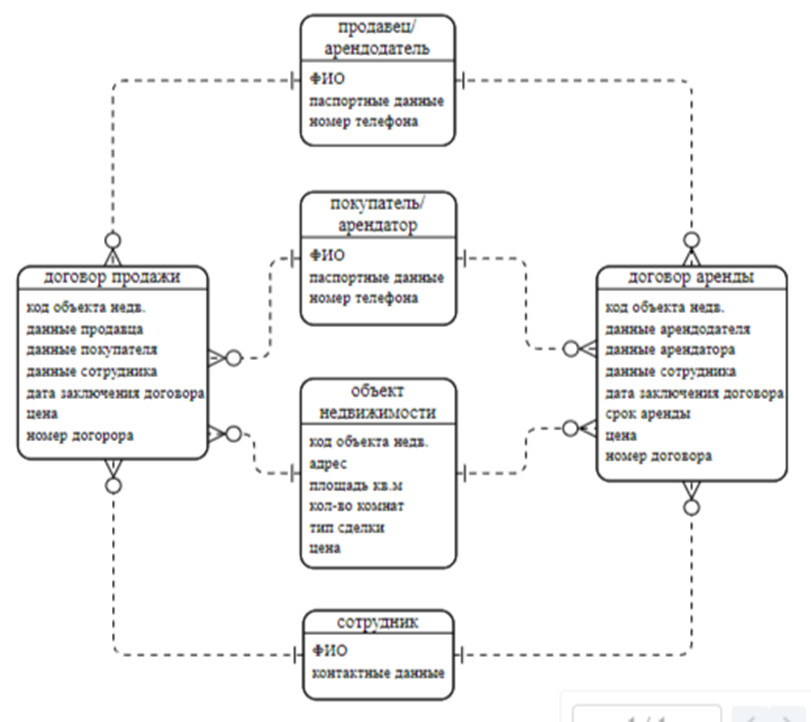
\includegraphics[width=1\linewidth]{er_diagr}
\caption{ER-диаграмма}
\label{ER_diagramma:image}
\end{figure}

\subsection{Логическое проектирование базы данных}

\subsubsection{Нормализация ER-модели данных}

Первая нормальная форма: каждый атрибут данной модели имеет только
одно значение.

Вторая форма: каждый атрибут зависит только от полного UID объекта.

Третья форма: каждый атрибут зависит только от UID своего объекта.

Объект «Продавец/арендодатель» соответствует 1NF, так как каждый атрибут имеет только одно значение.

Объект «Продавец/арендодатель» соответствует 2NF, так как каждый атрибут зависит от полного UID данного объекта.

Объект «Продавец/арендодатель» соответствует 3NF, так как каждый атрибут зависит только от UID данного объекта.

Объект «Покупатель/арендатор» соответствует 1NF, так как каждый атрибут имеет только одно значение.

Объект «Покупатель/арендатор» соответствует 2NF, так как каждый атрибут зависит от полного UID данного объекта.

Объект «Покупатель/арендатор» соответствует 3NF, так как каждый атрибут зависит только от UID данного объекта.

Объект «Объект недвижимости» соответствует 1NF, так как каждый атрибут имеет только одно значение.

Объект «Объект недвижимости» соответствует 2NF, так как каждый атрибут зависит от полного UID данного объекта.

Объект «Объект недвижимости» соответствует 3NF, так как каждый атрибут зависит только от UID данного объекта.

Объект «Сотрудник» соответствует 1NF, так как каждый атрибут имеет только одно значение.

Объект «Сотрудник» соответствует 2NF, так как каждый атрибут зависит от полного UID данного объекта.

Объект «Сотрудник» соответствует 3NF, так как каждый атрибут зависит только от UID данного объекта.

Объект «Договор продажи» соответствует 1NF, так как каждый атрибут имеет только одно значение.

Объект «Договор продажи» соответствует 2NF, так как каждый атрибут зависит от полного UID данного объекта.

Объект «Договор продажи» соответствует 3NF, так как каждый атрибут зависит только от UID данного объекта.

Объект «Договор аренды» соответствует 1NF, так как каждый атрибут имеет только одно значение.


На основе ER-модели данных в онлайн-сервисе Lucidcharts построена реляционная модель данных, показанная на рисунке \ref{exchange_scheme:image}.

\begin{figure}[H]
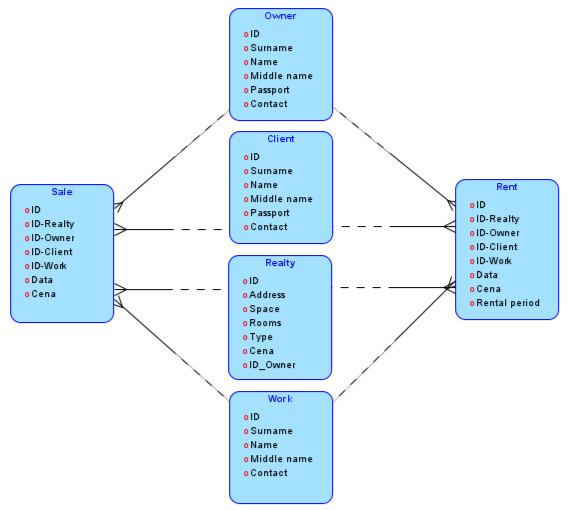
\includegraphics[width=0.8\linewidth]{model_dan}
\caption{Реляционная модель данных}
\label{exchange_scheme:image}
\end{figure}

Названия таблиц и названия столбцов каждой таблицы приведены в таблицах 3.1 -3.6.

\begin{xltabular}{\textwidth}{|l|l|X|X|}
	\caption{Владелец объекта недвижимости\label{owner:table}}\\ \hline
	\centrow Кеу Type & \centrow Optionality & \centrow Column name & \centrow Data type \\ \hline
	\thead{1} & \thead{2} & \centrow 3 & \centrow 4 \\ \hline
	\endfirsthead
	\thead{1} & \thead{2} & \centrow 3 & \centrow 4 \\ \hline
	\finishhead
	\ pk & * & Surname & TEXT \\ \hline
	& * & Name & TEXT \\ \hline
	& * & Middle name & TEXT \\ \hline
	& * & Passport & INTEGER \\ \hline
	& * & Contact & INTEGER \\ \hline
\end{xltabular}



\begin{xltabular}{\textwidth}{|l|l|X|X|}
	\caption{Клиент\label{client:table}}\\ \hline
	\centrow Кеу Type & \centrow Optionality & \centrow Column name & \centrow Data type \\ \hline
	\thead{1} & \thead{2} & \centrow 3 & \centrow 4 \\ \hline
	\endfirsthead
	\thead{1} & \thead{2} & \centrow 3 & \centrow 4 \\ \hline
	\finishhead
	\ pk & * & Surname & TEXT \\ \hline
	& * & Name & TEXT \\ \hline
	& * & Middle name & TEXT \\ \hline
	& * & Passport & INTEGER \\ \hline
	& * & Contact & INTEGER \\ \hline
\end{xltabular}



\begin{xltabular}{\textwidth}{|l|l|X|X|}
	\caption{Объект недвижимости\label{realty:table}}\\ \hline
	\centrow Кеу Type & \centrow Optionality & \centrow Column name & \centrow Data type \\ \hline
	\thead{1} & \thead{2} & \centrow 3 & \centrow 4 \\ \hline
	\endfirsthead
	\thead{1} & \thead{2} & \centrow 3 & \centrow 4 \\ \hline
	\finishhead
	\ pk & * & Address & TEXT \\ \hline
	& * & Space & TEXT \\ \hline
	& * & Rooms & INTEGER \\ \hline
	& * & Type & TEXT \\ \hline
	& * & Cena & INTEGER \\ \hline
	& * & ID owner & INTEGER \\ \hline
\end{xltabular}

\begin{xltabular}{\textwidth}{|l|l|X|X|}
	\caption{Сотрудник агентства\label{wort:table}}\\ \hline
	\centrow Кеу Type & \centrow Optionality & \centrow Column name & \centrow Data type \\ \hline
	\thead{1} & \thead{2} & \centrow 3 & \centrow 4 \\ \hline
	\endfirsthead
	\thead{1} & \thead{2} & \centrow 3 & \centrow 4 \\ \hline
	\finishhead
	\ pk & * & Surname & TEXT \\ \hline
	& * & Name & TEXT \\ \hline
	& * & Middle name & TEXT \\ \hline
	& * & Contact & INTEGER \\ \hline
\end{xltabular}

\begin{xltabular}{\textwidth}{|l|l|X|X|}
	\caption{Договор продажи\label{sale:table}}\\ \hline
	\centrow Кеу Type & \centrow Optionality & \centrow Column name & \centrow Data type \\ \hline
	\thead{1} & \thead{2} & \centrow 3 & \centrow 4 \\ \hline
	\endfirsthead
	\thead{1} & \thead{2} & \centrow 3 & \centrow 4 \\ \hline
	\finishhead
	\ pk & * & Realty & TEXT \\ \hline
	& * & Owner & TEXT \\ \hline
	& * & Client & TEXT \\ \hline
	& * & Work & TEXT \\ \hline
	& * & Data & DATE \\ \hline
	& * & Cena & INTEGER \\ \hline
\end{xltabular}

\begin{xltabular}{\textwidth}{|l|l|X|X|}
	\caption{Договор аренды\label{renta:table}}\\ \hline
	\centrow Кеу Type & \centrow Optionality & \centrow Column name & \centrow Data type \\ \hline
	\thead{1} & \thead{2} & \centrow 3 & \centrow 4 \\ \hline
	\endfirsthead
	\thead{1} & \thead{2} & \centrow 3 & \centrow 4 \\ \hline
	\finishhead
	\ pk & * & Realty & TEXT \\ \hline
	& * & Owner & TEXT \\ \hline
	& * & Client & TEXT \\ \hline
	& * & Work & TEXT \\ \hline
	& * & Data & DATE \\ \hline
	& * & Cena & INTEGER \\ \hline
	& * & Rental period & TEXT \\ \hline
\end{xltabular}
